%!TEX root = /Users/louis/Documents/PhD/Deliverables/Thesis/thesis.tex

\section{MDE Terminology and Principles}
\label{sec:mde_terms}
Software engineers using MDE construct and manipulate artefacts familiar from traditional approaches to software engineering (such as code and documentation) and, in addition, work with different types of artefact, such as \emph{models}, \emph{metamodels} and \emph{model transformations}. Furthermore, MDE involves new development activities, such as \emph{model management}. This section describes the artefacts and activities involved in MDE.

\subsection{Models}
\label{subsec:models}
Models are fundamental to MDE. \cite{kurtev04thesis} identifies many definitions of the term model, including the following: ``any subject using a system A that is neither directly nor indirectly interacting with a system B to obtain information about the system B, is using A as a model for B'' \cite{apostel60models}. ``A model is a representation of a concept. The representation is purposeful and used to abstract from reality the irrelevant details,'' \cite{starfield90model}. ``A model is a simplification of a system written in a well-defined language,'' \cite{bezivin01definition}. 

While there are many definitions of the term model, a common notion is that a model is a representation of the real-world \cite[pg12]{kurtev04thesis}. The part of the real-world represented by a model is termed the \emph{domain}, the \emph{object system} or, simply the \emph{system}. A further commonality is noted by \cite{kolovos06eol}: a model may have either a textual or graphical representation.

\cite{ackoff62scientific} defines \emph{analogous} models as those which share some characteristics and can be used in place of their object system. An aeroplane toy that can fly is an analogous model of an aeroplane. In computer science, models can be used to construct a computer system. A model of an object system, say the lending service of a library, might be used to decide the way in which data is stored on disk, or the way in which a program is to be structured.

\cite{jackson95software} proposes that the models constructed in computer science are analogous to two systems: the object system (e.g. the library lending service in the real-world) and the computer system (e.g. the software and hardware used to implement a library lending service). A model can be used to think about both the real system and the computer system. Figure~\ref{fig:jackson_model} illustrates this notion further. According to \cite{jackson95software}, a model is both the description of the domain (object system) and the machine (computer system). Computer scientists switch between \emph{designations} when using a model to think about the object system or to think about the software system.

\begin{figure}[htbp]
  \begin{center}
    \leavevmode
    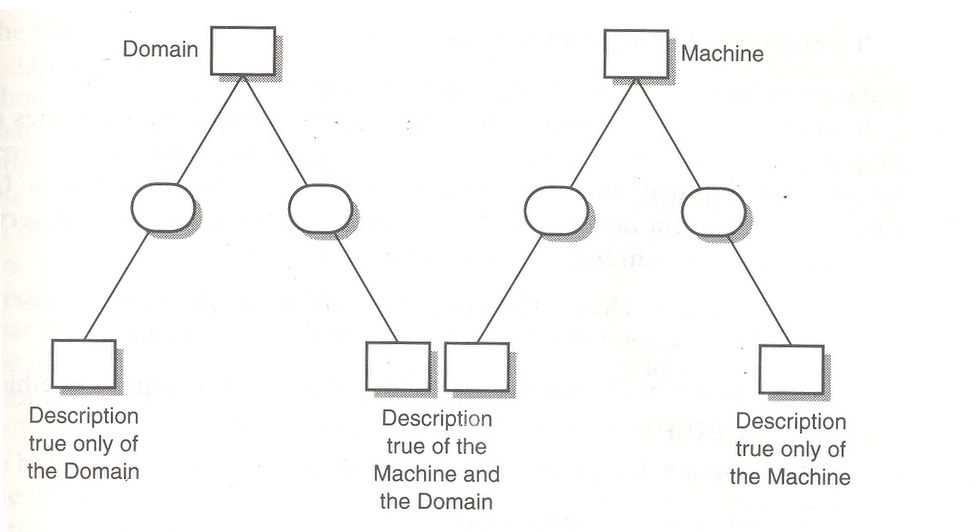
\includegraphics[width=10cm]{2.Background/images/jackson_model.png}
  \end{center}
  \caption[Jackson's definition of a model]{Jackson's definition of a model, taken from \cite[pg.125]{jackson95software}.}
  \label{fig:jackson_model}
\end{figure}

Models can be unstructured (for example, sketches on a piece of paper) or structured (conform to some well-defined set of syntactic and semantic constraints). In software engineering, models are used widely to reason about object systems and computer systems. MDE recognises this, and seeks to drive the development of computer systems from structured models.

\subsection{Modelling languages}
\label{subsec:modelling_languages}
In MDE, models are structured rather than unstructured \cite{kolovos09thesis}. A \emph{modelling language} is the set of syntactic and semantic constraints used to define the structure of a group of related models. In MDE, a modelling language is often specified as a model and, hence the term \emph{metamodel} is used in place of \emph{modelling language}.

\emph{Conformance} is a relationship between a metamodel and a model. A model \emph{conforms to} a metamodel when the metamodel specifies every concept used in the model definition, and the model uses the metamodel concepts according to the rules specified by the metamodel. Conformance can be described by a set of constraints between models and metamodels \cite{paige07metamodel}. When all constraints are satisfied, a model conforms to a metamodel. For example, a conformance constraint might state that every object in the model has a corresponding non-abstract class in the metamodel.

Metamodels facilitate model interchange and, therefore, interoperability between modelling tools.  For this reason, Evans recommends that software engineers ``use a well-documented shared language that can express the necessary domain information as a common medium of communication.'' \cite[pg377]{evans04domain}. To support this recommendation, Evans discusses the way in which chemists have collaborated to define a standardised language for describing chemical structures, Chemical Markup Language (CML)\footnote{\url{http://cml.sourceforge.net/}}. The standardisation of CML has facilitated interoperability between tools for specification, analysis and simulation.

A metamodel typically comprises three categories of constraint:

\begin{itemize}
	\item \textbf{The concrete syntax} provides a notation for constructing models that conform to the language. For example, a model may be represented as a collection of boxes connected by lines. A standardised concrete syntax enables communication. Concrete syntax may be optimised for consumption by machines (e.g. XML Metadata Interchange (XMI) \cite{xmi}) or by humans (e.g. the Unified Modelling Language (UML) \cite{uml212}).
	\item \textbf{The abstract syntax} defines the concepts described by the language, such as classes, packages, datatypes. The representation for these concepts is independent of the concrete syntax. For example, the implementation of a compiler might use an abstract syntax tree to encode the abstract syntax of a program (whereas the concrete syntax for the same language may be textual or graphical).
	\item \textbf{The semantics} identifies the meaning of the modelling concepts with respect to the domain. For example, consider a modelling language defined to describe genealogy, and another to describe flora. Although both languages may define a tree construct, the semantics of a tree in one is likely to be different from the semantics of a tree in the other. The semantics of a modelling language may be specified rigorously, by defining a reference semantics in a formal language such as Z \cite{z}, or in a semi-formal manner by employing natural language.
\end{itemize}

Concrete syntax, abstract syntax and semantics are used together to specify modelling languages. There are many other ways of defining languages, but this approach (first formalised in \cite{alvarez01mml}) is common in MDE: a metamodel is often used to define abstract syntax, a grammar or text-to-model transformation to specify concrete syntax, and code generators, annotated grammars or behavioural models to effect semantics.

\subsection{MOF: A metamodelling language}
\label{subsec:mof}
Software engineers using MDE can re-use existing -- and define new -- metamodels. To facilitate interoperability between MDE tools, the OMG has standardised a language for specifying metamodels, the Meta-Object Facility (MOF). Metamodels specified in MOF can be interchanged between MDE environments. Furthermore, modelling language tools are interoperable because MOF also standardises the way in which metamodels and their models are persisted to and from disk. For model and metamodel persistence, MOF prescribes XML Metadata Interchange (XMI), a dialect of XML optimised for loading, storing and exchanging models, and standardised by the OMG.

Because MOF is a modelling language for describing modelling languages, it is sometimes termed a metamodelling language. Part of the UML metamodel, defined in MOF, is shown in Figure~\ref{fig:mof}. As discussed in Section~\ref{sec:mde_tools}, different kinds of concrete syntax can be used for MOF. Figure~\ref{fig:mof}, for example, uses a concrete syntax similar to that of UML class diagrams. Specifically:

\begin{itemize}
 \item Modelling constructs are drawn as boxes. The name of each modelling construct is emboldened. The name of abstract (uninstantiable) constructs are italicised.
 \item Attributes are contained within the box of their modelling construct. Each attribute has a name, a type (prefixed with a colon) and may define a default value (prefixed with an equals sign).
 \item Generalisation is represented using a line with an open arrow-head.
 \item References are specified using a line. An arrow illustrates the direction in which the reference may be traversed. Labels are used to name and define the multiplicity of references.
 \item Containment references are specified by including a solid diamond on the containing end.
\end{itemize}

\begin{landscape}	
	\begin{figure}[htbp]
	  \begin{center}
	    \leavevmode
	    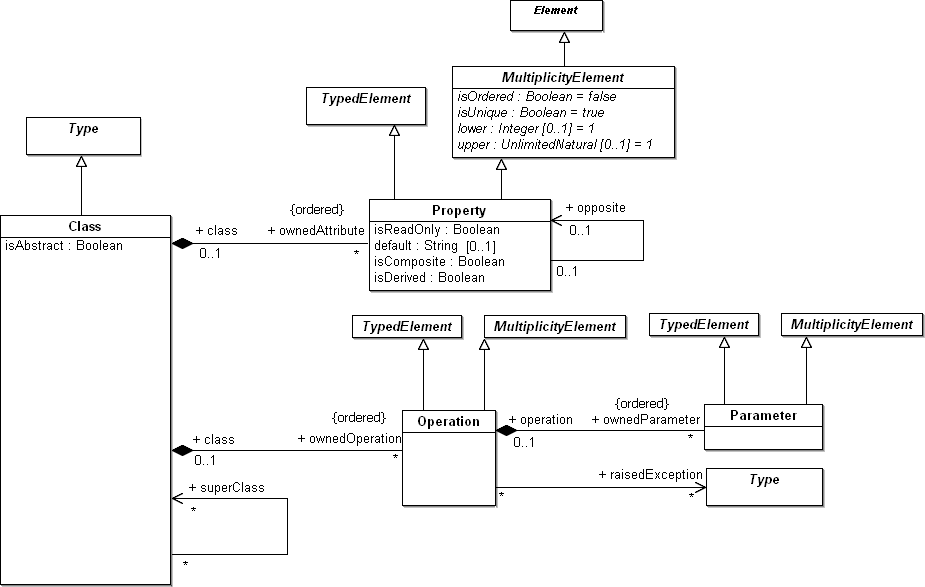
\includegraphics[scale=0.5]{2.Background/images/mof.png}
	  \end{center}
	  \caption[A fragment of the UML metamodel defined in MOF]{A fragment of the UML metamodel defined in MOF, from \cite{uml212}.}
	  \label{fig:mof}
	\end{figure}
\end{landscape}

Specifying modelling languages with a common metamodelling language, such as MOF, ensures consistency in the way in which modelling constructs are specified. MOF has facilitated the construction of interoperable MDE tools that can be used with a range of modelling languages. Without a standardised metamodelling language, modelling tools were specific to one modelling language, such as UML. In contemporary MDE environments, any number of modelling languages can be used together and manipulated in a uniform manner.

Furthermore, when modelling languages are specified without using a common metamodelling language, identifying similarities between modelling languages is challenging \cite[pg97]{frankel02mda}. The sequel discusses the way in which models and metamodels are used to construct systems in MDE.

\subsection{Model Management}
\label{sec:mde}
In MDE, models are \emph{managed} to produce software. \cite{melnik04thesis} first described \emph{model management} as a collection of operators for manipulating models. \cite{kolovos09thesis} explores a means for increasing the interoperability of model management operations. This thesis uses the term \emph{model management} to refer to development activities that manipulate models for the purpose of producing software. Model management activities typical in MDE, such as model transformation and validation, are discussed in this section. Section~\ref{sec:mde_methods} discusses MDE guidelines and methods, and describes the way in which model management activities are used together to produce software in MDE.

\subsubsection{Model Transformation}
\label{subsubsec:model_transformation}
Model transformation is a development activity in which software artefacts are derived from others, according to some well-defined specification. Three different types of model transformation are described in \cite{kleppe03mda,kolovos09thesis}. Model transformations are specified between modelling languages (model-to-model transformation), between modelling languages and textual artefacts (model-to-text-transformation) and between textual artefacts and modelling languages (text-to-model transformation). Each type of transformation has unique characteristics and tools, but share some common characteristics. The remainder of this section first introduces the commonalities and then discusses each type of transformation individually.

\paragraph{Common characteristics of model transformations}
The input to a transformation is termed its \emph{source}, and the output its \emph{target}. In theory, a transformation can have more than one source and more than one target, but not all transformation languages support multiple sources and targets. Consequently, much of the model transformation literature considers single source and target transformations.

\cite{czarnecki06survey} describe a feature model for distinguishing and categorising model transformation approaches. Two of the features are relevant to the research presented in this thesis, and are now discussed. 

\subparagraph{Source-target relationship} A \emph{new-target} transformation creates the target model afresh on each invocation, while an \emph{existing-target} transformation updates an existing model. Existing target transformations are used for partial (incremental) transformation and for preserving parts of the target model that are not derived from the source model.

\subparagraph{Domain language} Transformations specified between a source and a target model that conform to the same metamodel are termed \emph{endogenous} or \emph{rephrasings}, while transformations specified between a source and a target model that conform to different metamodels are termed \emph{exogenous} or \emph{translations}.

Endogenous, existing-target transformations are a special case of transformation and are termed \emph{refactorings}. Refactorings have been studied in the context of software evolution and are discussed more thoroughly in Chapter~\ref{LiteratureReview}.


\paragraph{Model-to-Model (M2M) Transformation} M2M transformation is used to derive models from others. By automating the derivation of models from others, M2M transformation has the potential to reduce the cost of engineering large and complex systems that can be represented as a set of interdependent models \cite{sendall03heart}. 

M2M transformations are often specified as a set of \emph{transformation rules} \cite{czarnecki06survey}. Each rule specifies the way in which a specific set of elements in the source model is transformed to an equivalent set of elements in the target model \cite[pg.44]{kolovos09thesis}.

Many M2M transformation languages have been proposed, such as the Atlas Transformation Language (ATL) \cite{jouault05transforming}, VIsual Automated model TRAnsformations (VIATRA) \cite{VIATRA} and the Epsilon Transformation Language (ETL) \cite{kolovos08etl}. Qu\-er\-ies/Vi\-ews/Tra\-nsfo\-rma\-ti\-ons (QVT) \cite{qvt} is a standard for M2M transformation. M2M transformation languages can be categorised according to their \emph{style}, which is either declarative, imperative or hybrid.

Declarative M2M transformation languages only provide constructs for mapping source to target model elements and, as such, are not computationally complete. Consequently, the scheduling of rules can be \emph{implicit} (determined by the execution engine of the transformation language). By contrast, imperative M2M transformation languages are computationally complete, but often require rule scheduling to be \emph{explicit} (specified by the user). Hybrid M2M transformation languages combine declarative and imperative parts, are computationally complete, and provide a mixture of implicit and explicit rule scheduling.

Declarative M2M transformation languages cannot be used to solve some categories of transformation problem \cite{patrascoiu04embedding}. Imperative M2M transformation languages are argued to be difficult to write and maintain \cite[pg.45]{kolovos09thesis}. Consequently, \cite{kolovos08etl} observes that hybrid languages, such as ATL, are presently believed to be more suitable for specifying model transformation than pure imperative or declarative languages.

An exemplar M2M transformation, written in the hybrid M2M transformation language ETL, is shown in Listing~\ref{lst:exemplar_m2m}. The source of the transformation is a state machine model, conforming to the metamodel shown in Figure~\ref{fig:state_machine_mm}. The target of the transformation an object-oriented model, conforming to the metamodel shown in Figure~\ref{fig:object_oriented_mm}. The transformation in Listing~\ref{lst:exemplar_m2m} comprises two rules.

\begin{figure}[htbp]
  \begin{center}
    \leavevmode
    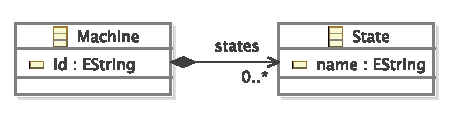
\includegraphics[scale=0.9]{2.Background/images/StateMachines.pdf}
  \end{center}
  \caption{Exemplar State Machine metamodel.}
  \label{fig:state_machine_mm}
\end{figure}

\begin{figure}[htbp]
  \begin{center}
    \leavevmode
    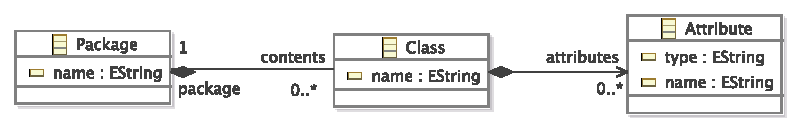
\includegraphics[scale=0.9]{2.Background/images/OO.pdf}
  \end{center}
  \caption{Exemplar Object-Oriented metamodel.}
  \label{fig:object_oriented_mm}
\end{figure}

The first rule (lines 1-7) is named \texttt{Machine2Package} (line 1) and transforms \emph{Machine}s (line 2) into \emph{Package}s (line 3). The body of the first rule (lines 5-6) specifies the way in which a \texttt{Package}, \texttt{p}, can be derived from a \texttt{Machine}, \texttt{m}. Specifically, the \texttt{name} of \texttt{p} is derived from the \texttt{id} of \texttt{m} (line 5), and the \texttt{contents} of \texttt{p} are derived from the \texttt{states} of \texttt{m} (line 6). 

The second rule (lines 9-16) transforms \texttt{State}s (line 10) to \texttt{Class}es (line 11). Additionally, line 13 contains a \emph{guard} to specify that the rule is only to be applied to \texttt{State}s whose \texttt{isFinal} property is \texttt{false}.

When executed, the transformation rules will be scheduled \textbf{implicitly} by the execution engine, and invoked once for each \texttt{Machine} and \texttt{State} in the source. On line 6 of Listing~\ref{lst:exemplar_m2m}, the built-in \texttt{equivalent()} operation is used to produce a set of \texttt{Class}es from a set of \texttt{State}s by invoking the relevant transformation rule. This is an example of \textbf{explicit} rule scheduling, in which the user defines when a rule will be called.

\begin{lstlisting}[caption={[M2M transformation in ETL]M2M transformation in the Epsilon Transformation Language \cite{kolovos08etl}}, label=lst:exemplar_m2m, language=ETL]
rule Machine2Package
	transform m : StateMachine!Machine
	to        p : ObjectOriented!Package {
		
	p.name     := 'uk.ac.york.cs.' + m.id;
	p.contents := m.states.equivalent();
}

rule State2Class
	transform s : StateMachine!State
	to        c : ObjectOriented!Class 
	
	guard: not s.isFinal {
		
	c.name := s.name + 'State';
}
\end{lstlisting}


\paragraph{Model-to-Text (M2T) Transformation} M2T transformation is used for model serialisation (enabling model interchange), code and documentation generation, and model visualisation and exploration.  In 2005, the Object Management Group (OMG)\footnote{\url{http://www.omg.org}} recognised the lack of a standardised M2T transformation with its M2T Language Request for Proposals\footnote{\url{http://www.omg.org/docs/ad/04-04-07.pdf}}. In response, various M2T languages were developed including MOFScript \cite{oldevik05toward}, the Epsilon Generation Language (EGL) \cite{rose08egl}, JET\footnote{\url{http://www.eclipse.org/modeling/m2t/?project=jet}} and XPand\footnote{\url{http://www.eclipse.org/modeling/m2t/?project=xpand}}.

Because M2T transformation is used to produce unstructured rather than structured artefacts, M2T transformation has different requirements to M2M transformation. For instance, M2T transformation languages often provide mechanisms for specifying sections of text that will be completed manually and must not be overwritten by the transformation engine.

\emph{Template}s are commonly used in M2T languages. Templates comprise \emph{static} and \emph{dynamic} sections. When the transformation is invoked, the contents of static sections are emitted verbatim, while dynamic sections contain logic and are executed.

An exemplar M2T transformation, written in EGL, is shown in Listing~\ref{lst:exemplar_m2t}. The source of the transformation is an object-oriented model conforming to the metamodel shown in Figure~\ref{fig:object_oriented_mm}, and the target is Java source code. The template assumes that an instance of \texttt{Class} is stored in the \texttt{class} variable.

\begin{lstlisting}[caption={[M2T transformation in EGL]M2T transformation in the Epsilon Generation Language \cite{rose08egl}}, label=lst:exemplar_m2t, language=EGL]
package [%=class.package.name%];

public class [%=class.name%] {
	[% for(attribute in class.attributes) { %]
	  private [%=attribute.type%] [%=attribute.name%];
	[% } %]
}
\end{lstlisting}

In EGL, dynamic sections are contained within \texttt{[\%} and \texttt{\%]}. \emph{Dynamic output} sections are a specialisation of dynamic sections contained within \texttt{[\%=} and \texttt{\%]}. The result of evaluating a dynamic output section is included in the generated text. Line 1 of Listing~\ref{lst:exemplar_m2t} contains two static sections (`\texttt{package}' and `\texttt{;}') and a dynamic output section (\texttt{[\%=class.package.name\%]}), and will generate a package declaration when executed.  Similarly, line 3 will generate a class declaration. Lines 4 to 6 iterate over every \texttt{attribute} of the \texttt{class}, outputting a field declaration for each \texttt{attribute}.


\paragraph{Text-to-Model (T2M) Transformation} T2M transformation is most often implemented as a parser that generates a model rather than object code. Parser generators such as ANTLR \cite{parr07antlr} can be used to produce a structured artefact (such as an abstract syntax tree) from text. T2M tools are built atop parser generators and post-process the structured artefacts to produce a model that can be managed with a particular modelling framework.

Xtext\footnote{\url{http://www.eclipse.org/Xtext/}} and EMFtext \cite{heidenreich09derivation} are contemporary examples of T2M tools that, given a grammar and a target metamodel, will automatically generate a parser that transforms text to a model.

An exemplar T2M transformation, written in EMFtext, is shown in Listing~\ref{lst:exemplar_t2m}. From the transformation shown in Listing~\ref{lst:exemplar_t2m}, EMFtext can be used to generate a parser that, when executed, will produce state machine models. For the input, \texttt{lift[stationary up down stopping emergency]}, the pa\-rser will produce a model containing one \texttt{Machine} with \texttt{lift} as its \texttt{id}, and five \texttt{State}s with the \texttt{name}s, \texttt{stationary}, \texttt{up}, \texttt{down}, \texttt{stopping}, and \texttt{em\-er\-ge\-ncy}.

Lines 1-2 of Listing~\ref{lst:exemplar_t2m} define the name of the parser and target metamodel. Line 3 indicates that parser should first seek to construct a \texttt{Machine} from the source text. Lines 5-9 define rules for the lexer, including a rule for recognising \texttt{IDENTIFIER}s (represented as alphabetic characters).

Lines 11-14 of Listing~\ref{lst:exemplar_t2m} are key to the transformation. Line 11 specifies that a \texttt{Machine} is constructed whenever an \texttt{IDENTIFIER} is followed by a \texttt{LBRACKET} and eventually a \texttt{RBRACKET}. When constructing a \texttt{Machine}, the first time an \texttt{IDENTIFIER} is encountered, it is stored in the \texttt{id} attribute of the \texttt{Machine}. The \texttt{states*} statement on line 12 indicates that, before matching a \texttt{RBRACKET}, the parser is permitted to transform subsequent text to a \texttt{State} (according to the rule on line 13) and store the resulting \texttt{State} in the \texttt{states} reference of the \texttt{Machine}. The asterisks in \texttt{states*} indicates that any number of \texttt{State}s can be constructed and stored in the \texttt{states} reference.

\begin{lstlisting}[caption=T2M transformation in EMFtext, label=lst:exemplar_t2m, language=EMFtext]
SYNTAXDEF statemachine
FOR <statemachine>
START Machine

TOKENS {
	DEFINE IDENTIFIER $('a'..'z'|'A'..'Z')*$;
	DEFINE LBRACKET $'['$;
	DEFINE RBRACKET $']'$;
}

RULES {
	Machine ::= id[IDENTIFIER] LBRACKET states* RBRACKET  ;
	State ::= name[IDENTIFIER] ;
}
\end{lstlisting}

\subsubsection{Model Validation}
\label{subsubsec:model_validation}
Model validation provides a mechanism for managing the integrity of the software developed using MDE. A model that omits information is said to be \emph{incomplete}, while related models that suggest differences in the underlying phenomena are said to be \emph{contradicting} \cite{kolovos09thesis}. Incompleteness and contradiction are two examples of \emph{inconsistency}. In MDE, inconsistency is detrimental, because, when artefacts are automatically derived from each other, the inconsistency of one artefact might be propagated to others. Model validation is used to detect, report and reconcile inconsistency throughout a MDE process.

\cite{kolovos09thesis} observes that inconsistency detection is inherently pattern-based and, hence, higher-order languages are more suitable for model validation than so-called ``third-generation'' programming languages (such as Java). The Object Constraint Language (OCL) \cite{ocl2} is an OMG standard that can be used to specify consistency constraints on UML and MOF models. OCL cannot be used to specify inter-model constraints, unlike the xlinkit toolkit \cite{nentwich2003flexible} and the Epsilon Validation Language (EVL) \cite{kolovos08evl}.

An exemplar model validation constraint, written in EVL, is shown in Listing~\ref{lst:exemplar_validation}. The constraint validates state machine models that conform to the metamodel shown in Figure~\ref{fig:state_machine_mm}. The constraint shown in Listing~\ref{lst:exemplar_validation} is defined for \texttt{State}s (line 1), and checks that there exists some transition whose source or target is the current state (line 4). When the check part (line 4) is not satisfied, the message part (line 6) is displayed. When executed, the EVL constraint will be invoked once for every \texttt{State} in the model. The keyword \texttt{self} is used to refer to the particular \texttt{State} on which the constraint is currently being invoked.

\begin{lstlisting}[caption={[Model validation in EVL]Model validation in the Epsilon Validation Language}, label=lst:exemplar_validation, language=EVL]
context State {
	constraint NoStateIsAnIsland {
		check:
			Transition.all.exists(t | t.source == self or t.target == self)
		message:
		  'The state ' + self.name + ' has no transitions.'
	}
}
\end{lstlisting}

\subsubsection{Further model management activities}
In addition to model transformation and validation, further examples of model management activities include model comparison (e.g. \cite{kolovos09ecl}), in which a \emph{trace} of similar and different elements is produced from two or more models, and model merging or weaving (e.g. \cite{kolovos07eml}), in which two or more models are combined to produce a unified model.

Further activities, such as model versioning and tracing, might be regarded as model management but, in the context of this thesis, are considered as evolutionary activities and as such are discussed in Chapter~\ref{LiteratureReview}.

\subsection{Summary}
This section has introduced the terminology and principles necessary for discussing MDE in this thesis. Models provide abstraction, capturing necessary and disregarding irrelevant details. Metamodels provide a structured mechanism for describing the syntactic and semantic rules to which a model must conform. Metamodels facilitate interoperability between modelling tools. MOF, the OMG standard metamodelling language, enables the development of tools that can be used with a range of metamodels, such as model management tools. Throughout an MDE process, models are manipulated to produce other development artefacts using model management activities such as model transformation and validation. Using the terms and principles described in this section, the ways in which MDE is performed in practice are now discussed.